% options:
% thesis=B bachelor's thesis
% thesis=M master's thesis
% czech thesis in Czech language
% english thesis in English language
% hidelinks remove colour boxes around hyperlinks

\documentclass[thesis=M,english]{FITthesis}[2012/10/20]

\usepackage[utf8]{inputenc} % LaTeX source encoded as UTF-8

\usepackage{graphicx} %graphics files inclusion

% \usepackage{subfig} %subfigures
% \usepackage{amsmath} %advanced maths
% \usepackage{amssymb} %additional math symbols

\usepackage{dirtree} %directory tree visualisation


% list of acronyms
\usepackage[acronym,nonumberlist,toc,numberedsection=autolabel,nomain]{glossaries}
\iflanguage{czech}{\renewcommand*{\acronymname}{Seznam pou{\v z}it{\' y}ch zkratek}}{}
\makeglossaries

\newcommand{\tg}{\mathop{\mathrm{tg}}} %cesky tangens
\newcommand{\cotg}{\mathop{\mathrm{cotg}}} %cesky cotangens


% % % % % % % % % % % % % % % % % % % % % % % % % % % % % % % % % % % 
% % % % % % % % % % % % % % % % % % % % % % % % % % % % % % % % % % % 
\department{Department of theoretical computer science}
\title{Detection of DNS Anomalies via Data Mining Analysis of Network Traffic}
\authorGN{Michal} %author's given name/names
\authorFN{Pohořelý} %author's surname
\authorWithDegrees{Bc. Michal Pohořelý} %author's name with academic degrees
\supervisor{Mgr. Rudolf Blažek, Ph.D.}
\acknowledgements{I would like to thank my supervisor Mgr. Rudolf Blažek for support during writing this thesis.}
\abstractCS{Tato práce se zabývá anomáliemi v DNS provozu a jejich identifikací a klasifikací. Součástí práce je také rozbor metod pro použití při klasifikace. Hlavní částí práce je výběr a implementace vybrané metody pro klasifikaci DNS anomálií s příslušnými výsledky.}
\abstractEN{This thesis is concerned with anomalies in DNS traffic and their identification and clasification. Part of this theses is also ananalysis of methods acceptable for classification. The main part is selection and implementation of selected method for classification of DNS anomalies with their results.}
\placeForDeclarationOfAuthenticity{Prague} %where you have signed the declaration
\keywordsCS{DNS, anomálie, datamining, neuronové sítě, CZ.NIC.}
\keywordsEN{DNS, anomalies, datamining, neural nets, CZ.NIC.}
\declarationOfAuthenticityOption{4} %select as appropriate, according to the desired license

\begin{document}

\newacronym{LZW}{LZW}{Lempel Ziv Welch}
\newacronym{RLE}{RLE}{Run-Length Encoding}

\begin{introduction}

\end{introduction}

\chapter{DNS - Domain Name System}\label{dns}
Domain Name System is a hierarchical distributed naming system for any resource connected to the Internet \cite{wik14}. You can imagine its function like a phone book what is translating human friendly domain names (e.g. www.nic.cz) to IP address. IP address is the identification of every computer or other device connected to the Internet and must be unique (except of NAT). IPv4 is 32 bits long and is composed of four octets like numbers in range of values 0 to 255 delimited by dots (e.g. 217.31.205.50). So you can see that form in IP address is much more difficult to memorize than www.nic.cz. And more difficult is situation in IPv6 which is 128 bits long and is composed of eight 16-bits hexadecimal values delimited by colon (e.g. 2001:1488:800:400::130). This is the main reason why the DNS is being used.

\section{Normal DNS Usage}
\subsection{Components of DNS}
There are three major parts of DNS \cite{Moc87}
\begin{itemize}
\item The domain name space and resource records which are specifications for a tree tree structured name space and data associated with the names. Every node of a tree contains a subset of information. Query operation are trying to extract information from a particular subset. Query contains the domain name and DNS type.
\item Names servers are server programs which hold information about the domain tree's structure and set information. They can have information about any part of domain tree but practicaly they serve only a part of domain space. They also have a pointer to other name servers to serve any part of domain space. If the server knows everything about the subset of some part of domain space we call it authoritative name server.
\item Resolvers are client applications that are extracting information from name servers in responce to client requests. They need to have access at least to one name server. Resolver asks the name server and name server give him an answer or link to next name server where the information should be found.
\end{itemize}

\subsection{DNS record}
Structure of DNS record \cite{Moc87a}

\begin{itemize}
\item NAME - owner name, the name of the node to which this resource record pertains
\item TYPE - 16bit type code
\item CLASS - 16bit class code
\item TTL - 32bit time interval of record lifetime
\item RDLENGTH - 16bit length of RDATA
\item RDATA - variable length string that describes the resource
\end{itemize}

\subsection{DNS resolution}
DNS resolution is proccess of finding an IP address of requesting host. The usual scenario is on Figure:\ref{fig:dns_res}

\begin{figure}[h]
  \centering
  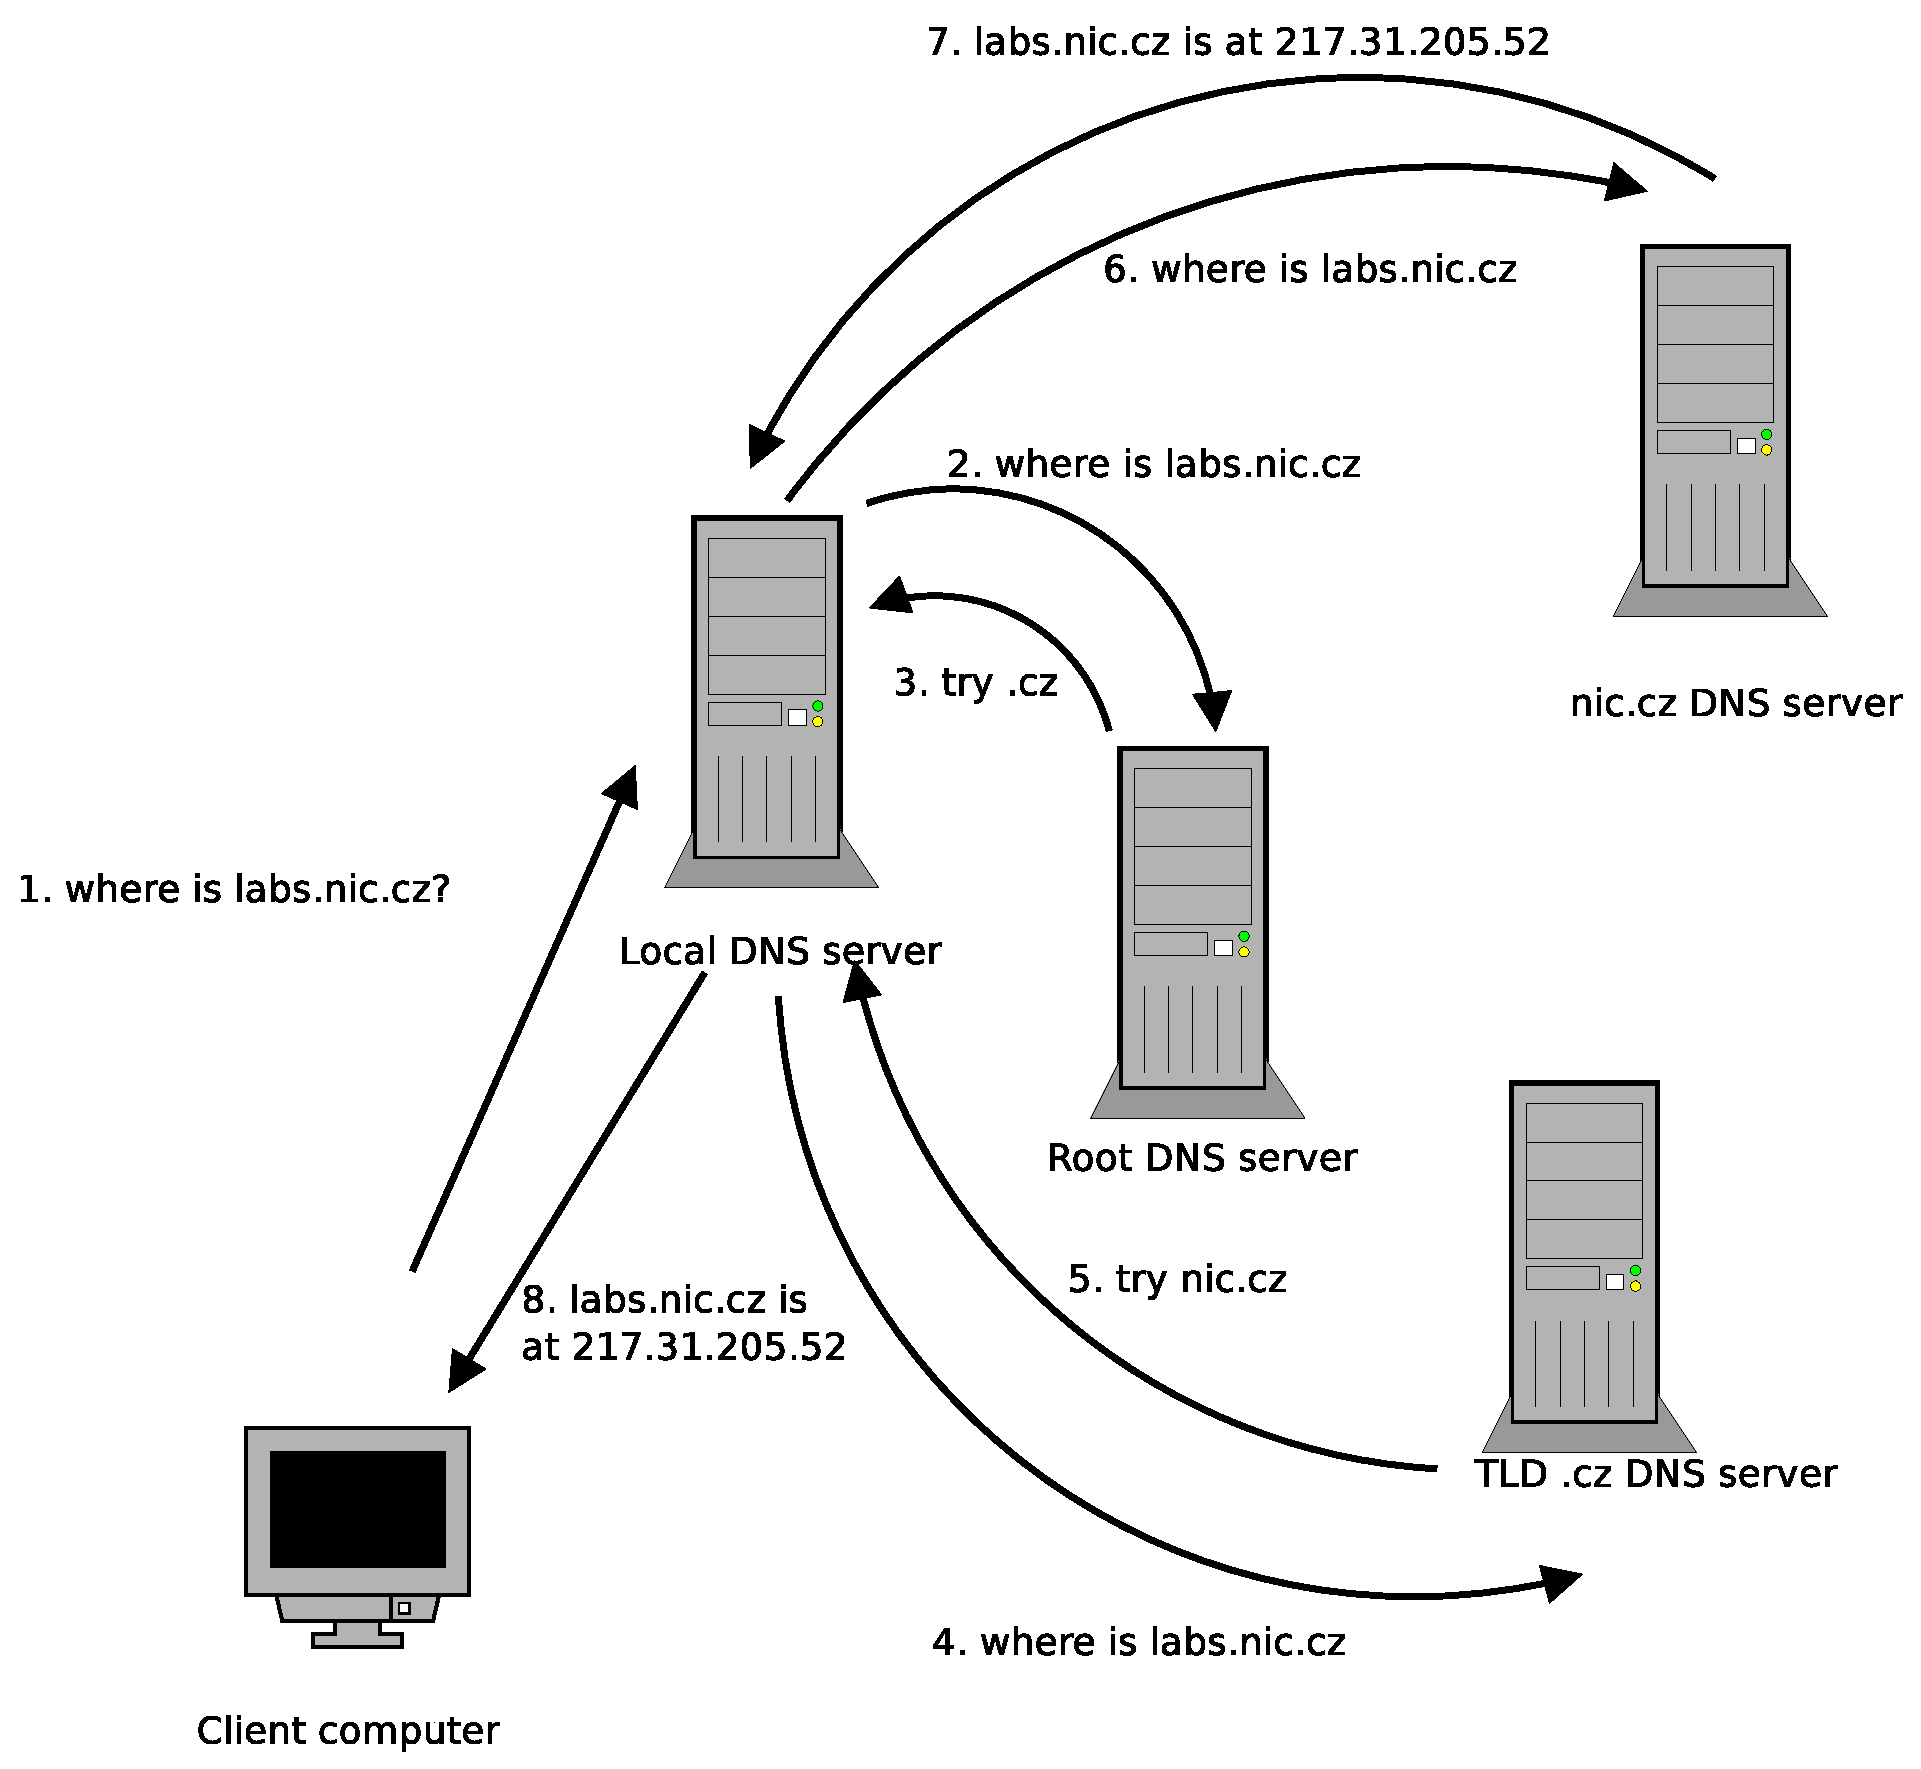
\includegraphics[width=15cm]{./img/dns_resolution}
  \caption{Resolution of requsted IP address}
  \label{fig:dns_res}
\end{figure}


At first client asks his local DNS server (usually ISP DNS server). If the local DNS server doesn't know the answer he will then ask root DNS server. He will give him answer where to find the TLD DNS server for .cz domain. Local DNS server will ask this TLD DNS server and he will get an answer where to find nic.cz DNS server. Local DNS server will continue there and he will get an exact answer with IP address of labs.nic.cz and he will give to client.
\section{Anomalous DNS Traffic}
Anomalous traffic is when DNS protocol is being used for any other reason than for translating domain names to IP address or reverse. We can then split this traffic to following groups.
\chapter{Analysis of DNS Attacks}

\section{DoS Attacks}
DoS attacks can be classified into two major categories \cite{KamMosGen08}
\begin{itemize}
\item Try to exploit vulnerabilities in the implemented software (ping of death). This type of vulnerability is mostly fixed in new devices and nowadays is the flooding attack more common.
\item Try to overhelm system resources i.e. memory, CPU, network bandwith. In this type of attack is usually used the amplification DNS attack that lies in the fact that DNS respond messages may be substantially larger than DNS query messages. Attacker sends DNS request with victims IP address and the respond will deliver to victims network. This is because open recursive DNS servers are not checking request validity.
\end{itemize}
\section{MiM Attacks}
This type of attack is used to redirect user to fake website to gain private information of the client. When the client attempts to connect the website he sends a DNS request. The attacker captures this request and sends a fake answer with IP address with his webserver. Victim will start to communicate with attackers web server instead of the real one. \cite{BaiHuSon11}
\section{DNS Tunelling}
This is the technic when the attacker wants to circumvent a security policies. Typical example is to illegally browse the web when access fee is requested. DNS requests are usually not filtered on firewall so this communication is open. Attacker encapsulates his data into DNS packets. \cite{EllZurSpe13}
\section{Botnets}
Malicious botnets are distributed computing platforms predominantly used for illegal actvities such as launching Distributed Denial of Service (DDoS) attacks, sending spam, trojan and phishing emails, illegally ditributing pirated media and software, force distribution, stealing information and computing resource, e-business extortion, performing click fraud, and identity theft. Victim's computer beacame a part of botnet usually by launching some infected application.\cite{FeiShaRam09}
\section{Other DNS Related Attacks}

\chapter{Methods of DNS Attack Detection and Classification}

\section{Ad-hoc Methods}
\section{Signatures}
\section{Data-Mining Methods}
\subsection{Random Forest}
\subsection{Neural Nets}
\section{Statistical Methods}

\chapter{Description of Selected Method}

\chapter{Application Design}

\chapter{Implementation}

\chapter{Measurements and Testing}

\begin{conclusion}
\end{conclusion}

\nocite{*}

\bibliographystyle{iso690.bst}
\bibliography{zotbib}

\appendix

\printglossaries

\chapter{Contents of CD}\label{app:CDcontent}

Visualise the contents of enclosed media. Use of \verb|dirtree| is recommended. Note that directories src and text with appropriate contents are mandatory.


\begin{figure}
	\dirtree{%
		.1 readme.txt\DTcomment{the file with CD contents description}.
		.1 data\DTcomment{the data files directory}.
		.2 graphs\DTcomment{the directory of graphs of experiments}.
		.3 *.eps\DTcomment{the B/W graphs}.
		.3 *.png\DTcomment{the color graphs}.
		.3 *.dat\DTcomment{the graphs data files}.
		.1 exe\DTcomment{the directory with executable WBDCM program}.
		.2 wbdcm\DTcomment{the WBDCM program executable (UNIX)}.
		.2 wbdcm.exe\DTcomment{the WBDCM program executable (Windows)}.
		.1 src\DTcomment{the directory of source codes}.
		.2 wbdcm\DTcomment{the directory of WBDCM program}.
		.3 Makefile\DTcomment{the makefile of WBDCM program (UNIX)}.
		.2 thesis\DTcomment{the directory of \LaTeX{} source codes of the thesis}.
		.3 figures\DTcomment{the thesis figures directory}.
		.3 *.tex\DTcomment{the \LaTeX{} source code files of the thesis}.
		.1 text\DTcomment{the thesis text directory}.
		.2 thesis.pdf\DTcomment{the Diploma thesis in PDF format}.
		.2 thesis.ps\DTcomment{the Diploma thesis in PS format}.
	}
\end{figure}


\end{document}
